\begin{savequote}[75mm]
The technique of combinatorics made it possible to establish relationships, which could go from the first flute to the last double bass: very tense connections throughout the work, nothing evident to the ear or the eye, but important to maintain the structural fact. [...] At a macroscopic level it was possible for us to see the whole work from afar and give an explanation of the \emph{why} of a particular note, although the composer could vary something he did not like.
\qauthor{Francisco Guerrero Marín\footnote{\citet[175]{guerrero-quote}}}
\end{savequote}

\chapter{\textit{Alu} (2024) for Sinfonietta}
\label{Chapter4}
% \lettrine[lines=2,slope=-2pt,nindent=2pt]{\textcolor{SchoolColor}{A}}{lu, for sinfonietta,}

\lettrine[lines=3]{\setmainfont{GoudyInitialen}[Path=./fonts/, Extension = .ttf]\color{printGreen}A}{lu for sinfonietta,} just like \textit{Polillas,} was influenced directly by my study of the preceding works. The large-scale formal architecture is informed by a fusion of the approaches of Guerrero and Bača, the material definitions are more closely related to those employed by Guerrero, and the freely experimental yet structural nature of the harmonic language seen in Barraqué is the spiritual successor to the harmonic language of this work. \textit{Alu} is perhaps also in dialogue with my 2018 work for 21 saxophones given the (admittedly naïve) title \textit{GUERRERO}, representing one of my earliest acknowledged compositions.

When adapting one's compositional technique to the environment afforded by computation, there appears to be a trend toward the dissolution of motivicity, or at least rhythmic directionality: it is trivial to produce page upon page of related rhythmic materials for even a large ensemble in just a few short moments; however, wallpapering the resonant chamber of a concert hall with unending, anonymous textures is rarely compelling composition. This is not only a common pitfall for composers thrust for the first time into the potentially alienating arena of musical formalization, this was my personal struggle when I first adopted such a compositional process. My composition \textit{GUERRERO,} while remaining an official component of my œuvre, can certainly be read as a ``wallpapering'' listening experience.

As previously hinted, my works \textit{Torlannol} and \textit{Infiorescenze} portend a shift in my musical language away from the mass textures which characterize much of my music until now. It felt fitting then, here at the end of my doctoral studies, to revisit the possibilities of the swarming mass textures of \textit{GUERRERO} made particularly powerful in the context of a large ensemble such as a sinfonietta, now also making use of my newly established criteria for strong formal structures.

\section{Desiderata}

I have a tendency to title compositions with a single word, often in a language other than English. This could be read as a banal exoticism; however, the habit is the result of a twofold æsthetic pressure. I am not typically comfortable deploying titles conventionally attributed to classical genres such as ``sonata,'' ``symphony,'' or ``concerto,'' but referring to a work as ``Composition no.1 for orchestra'' as was popular for a time in the 1950's feels unremarkable. Neither am I comfortable with extramusical meaning being used to justify the musical discourse of a work and my relationship to text in music is particularly fraught. What then am I to do? It has been my practice to compromise on the subject of extramusical meaning by using a creative word or phrase as a title and writing that title in a language, or better yet a writing system, other than what is native to me, placing that extramusical meaning at a distance. There is however, an extra-musical significance to the title and the basic gestural qualities to each material.

The title of the work \textit{Alu}, a word found on many runestones, does not have a clear definition. It is thought to mean ``ale'' (i.e. alcohol) and is used to mean ``bravery,'' ``strength,'' ``protection,'' as well as many other translations. The inscription of Alu becomes an amulet over time, appearing in isolation or in an abstracted context. Runestones can be notoriously difficult to decipher. Various forms of cryptography are used in runestone carving. A famous use of cipher runes can be found on the Rökstenen carved around 800 CE. Henrik Williams, in his book ``Rökstenen och världens undergång,'' illustrates a possible interpretation of the content of the stone as well as an interpretation of the kennings and cipher runes on the stone.

In reaching for a relationship to runestones, I am not attempting to force, as has unfortunately been historically precedent, a white ethno-nationalist æsthetic. The Armanen runes invented in 1906 and various icons in Nazi symbology draw on runes to project a false pagan history rooted in Northern Europe in an attempt to distance European Christianity's relationship to Judaism and other aspects of Semitic history. While the use of runes, especially typography which features either the Elder or Younger Futhark, carries the baggage of a white ethno-nationalist connotation,\footnote{Perhaps especially so in the current political climate of the United States} my admiration for the carving of runestones lies in the subterfuge of this particular literate tradition.

Material \boxed{\text{A}} is meant to be reminiscent of the sound of chiseling and is eventually meant to be transfigured into the ticking of a clock. Material \boxed{\text{B}} is meant to illustrate a kind of entropy on the geologic time scale: earth erodes and plant life encroaches on the edifices erected by humanity. Material \boxed{\text{C}} is perhaps the sound of the growing plant life itself or the falling rain. Something in this material echoes the revving of the engine of a sports car in the distant future relative to the carving of a runestone. Material \boxed{\text{D}} was meant to be the scraping of a stone being dragged from the location of its carving to the final, permanent resting place. The rest of the materials have no explicit, literal meaning. A runestone was typically erected as a memorial to the passing of a loved one or a momentous historical occasion. Here, I erect my stone in honor of the end of a particular time in my life as a student and tell myself ``alu: be protected and have courage.''

\section{Inherited Techniques}

Many of the techniques used to compose this piece were directly inherited from the composers described earlier in this dissertation. The large-scale structure is influenced by Guerrero's use of steiner systems. The rhythmic language of the piece is influenced bu Bača's rhythm-making techniques.

\section{Formal Permutations}

In \textit{Polillas,} I derived certain formal structures from the Fano plane, leading to the decision to use seven basic materials. In \textit{Alu,} as a result of my desire to use more than seven materials, I derive structures from the Affine plane. The Affine plane is a solution to Steiner system S(2, q, q\textsuperscript{2}). The system S(2, 3, 9) features arrangements of nine elements and resolves to S=((ABC, BDI, DEF, ECG, CFI, FGB, GHI, HBE, EAI, ADG, DHC, HFA)). The plane contains n\textsuperscript{2} points, each point is contained in n+1 lines, and there are n\textsuperscript{2}+n lines.

\begin{figure}[H]
    \centering
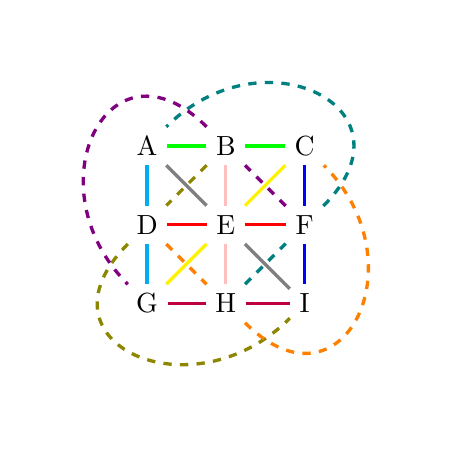
\begin{tikzpicture}
    \node(1) {A};
    \node[right of=1] (2) {B};
    \node[right of=2] (3) {C};
    \node[below of=1] (4) {D};
    \node[below of=2] (5) {E};
    \node[below of=3] (6) {F};
    \node[below of=4] (7) {G};
    \node[below of=5] (8) {H};
    \node[below of=6] (9) {I};
    \draw[-, very thick]
    (1) edge[green] (2)
    (2) edge[green] (3)
    (4) edge[red] (5)
    (5) edge[red] (6)
    (7) edge[purple] (8)
    (8) edge[purple] (9)
    (3) edge[yellow] (5)
    (5) edge[yellow] (7)
    (1) edge[gray] (5)
    (5) edge[gray] (9)
    (3) edge[blue] (6)
    (6) edge[blue] (9)
    (1) edge[cyan] (4)
    (4) edge[cyan] (7)
    (2) edge[pink] (5)
    (5) edge[pink] (8)
    (2) edge[olive, dashed] (4)
    (4) edge[olive, dashed, out=225, in=225, looseness=2] (9)
    (4) edge[orange, dashed] (8)
    (8) edge[orange, dashed, out=315, in=315, looseness=2] (3)
    (8) edge[teal, dashed] (6)
    (6) edge[teal, dashed, out=45, in=45, looseness=2] (1)
    (6) edge[violet, dashed] (2)
    (2) edge[violet, dashed, out=135, in=135, looseness=2] (7); 

\end{tikzpicture}
    \caption{Affine Plane}
    \label{fig:affine-plane}
\end{figure}

Five main material collections derive from a re-partitioning of the plane into ((ABC), (BDI, DEF), (ECG, CFI, FGB), (GHI, HBE, EAI), (ADG, DHC, HFA)). I then simplify each partition to (ABC, BDIEF, ECGFIB, GHIBEA, HFADCG). I calculate combinations from each partition from size 1-4 and select those which I feel are musically compelling to produce the sequence ((A, B, A, BC, A), (B, BD, BIE, BDEF, BF), (CF, C, CGI, CB, ECFB, C), (HB, H, HIE, HA, GHBA, H), (A, AC, HADC, G, GC, GCD, GCDA, A)). Each of the five main sequences has a primary material: sequence one primarily features \boxed{\text{A}}, two features \boxed{\text{B}}, three features \boxed{\text{C}}, four features \boxed{\text{H}}, and sequence five emphasizes \boxed{\text{A}} at the beginning and end, but emphasizes \boxed{\text{G}} in the center. Sequences three and four are arranged as ciphers of one another. They share the same structure yet expose different materials.

\subsection{Main Sections}

In composing \textit{Alu,} I wanted to take several risks by using unfamiliar composing strategies. First, the work is divided into a main binary structure, distinct from my typical narrative structures. The first section represents one long, stable glow, perhaps under the metaphorical haze of historical time. The materials are meant to freely overlap, coexisting rather than having an oppositional or teleological relationship. The second section is meant to more rigidly contrast a wide variety of materials. The materials of the second section, in contrast to the first, are meant to refuse development.

The formal design of \textit{Alu} begins with the definition of 5 proportions which are used to calculate the duration of each main section of the work. The proportions divide \textit{Alu} into an \textbf{introduction} with a proportional value of $1$, \textbf{section A} with a proportional value of $16 \div ϕ$, \textbf{section B} with a proportional value of $16$, and a \textbf{coda} with a proportional value of $\frac{16 \div ϕ}{ϕ}$. \textbf{Section B} subdivides into two sections to allow for the kind of structural repetition with different materials as previously seen in \textit{Polillas}, resulting in individual proportions of $8$. See figure \ref{fig:main-sections}.

\begin{figure}[p]
    \centering
    \rotatebox{90}{
    \resizebox{0.9\textheight}{!}{
\begin{tikzpicture}[
every edge quotes/.style = {font=\normalsize, rectangle, draw, fill=white}
                    ]
    \draw[pattern=crosshatch dots, pattern color=gray] (0,0) rectangle (1,1);
    \draw[pattern=crosshatch, pattern color=blue] (1,0) rectangle (11,1);
    \draw[pattern=north east lines, pattern color=orange] (11,0) rectangle (19,1);
    \draw[pattern=north west lines, pattern color=orange] (19,0) rectangle (27,1);
    \draw[pattern=crosshatch dots, pattern color=gray] (27,0) rectangle (33.25,1);

    \node (n1) at (0.5,1.25) {Intro};
    \node (n2) at (1.5,1.25) {A};
    \node (n3) at (11.5,1.25) {B1};
    \node (n4) at (19.5,1.25) {B2};
    \node (n5) at (27.5,1.25) {Coda};

    \node (n6) at (0.5,-1.25) {$1$};
    \node (n7) at (6,-1.25) {$\frac{16}{ϕ} \approx 10$};
    \node (n8) at (15,-0.25) {$8$};
    \node (n9) at (23,-0.25) {$8$};
    \node (n10) at (19,-1.25) {$8 + 8 = 16$};
    \node (n11) at (30.125,-1.25) {$\frac{16 \div ϕ}{ϕ} \approx 6.25$};

    \draw[<->, thick]
    (n7) edge[black, out=-45, in=-135, looseness=0.25, "main binary"] (n10)
    (n3) edge[black, out=45, in=135, looseness=0.25, "structural repetition"] (n4)
    ;

\end{tikzpicture}
}
}
    \caption{Basic Formal Plan}
    \label{fig:main-sections}
\end{figure}

After these proportional factors are derived, they are used to calculate the duration in seconds of each main section through the use of equation \ref{eq:guerrero-proportions}.

\begin{figure}[H]
    \centering
    1 + 10 + 8 + 8 + 6.25 = 33.25
    \caption{Proportions of main sections of \textit{Alu}}
    \label{fig:alu-props}
\end{figure}

So to perform the duration calculation on these proportions we obtain the following durations with a desired total duration of 1200'' assuming a basic tempo of \quarterNote = 60.

\begin{equation}
    D_1 = \frac{(1 \cdot 1200)}{33.25} \approx 36'' = 0.6' (\text{c.9 mm of \lilyTimeSignature{4}{4})}
\end{equation}

\begin{equation}
    D_2 = \frac{(10 \cdot 1200)}{33.25} \approx 361'' = 6' (\text{c.90 mm of \lilyTimeSignature{4}{4})}
\end{equation}

\begin{equation}
    D_3 = \frac{(8 \cdot 1200)}{33.25} \approx 289'' = 4.8' (\text{c.72 mm of \lilyTimeSignature{4}{4})}
\end{equation}

\begin{equation}
    D_4 = \frac{(8 \cdot 1200)}{33.25} \approx 289'' = 4.8' (\text{c.72 mm of \lilyTimeSignature{4}{4})}
\end{equation}

\begin{equation}
    D_5 = \frac{(6.25 \cdot 1200)}{33.25} \approx 226'' = 3.8' (\text{c.56 mm of \lilyTimeSignature{4}{4})}
\end{equation}

Each subsection of \textbf{B} is divided by the same set of proportions.

\begin{equation}
    d_1 = \frac{(1 \cdot 289)}{33.25} \approx 9'' = 0.15' (\text{c.2 mm of \lilyTimeSignature{4}{4})}
\end{equation}

\begin{equation}
    d_2 = \frac{(10 \cdot 289)}{33.25} \approx 87'' = 1.45' (\text{c.22 mm of \lilyTimeSignature{4}{4})}
\end{equation}

\begin{equation}
    d_3 = \frac{(8 \cdot 289)}{33.25} \approx 70'' = 1.167' (\text{c.17 mm of \lilyTimeSignature{4}{4})}
\end{equation}

\begin{equation}
    d_4 = \frac{(8 \cdot 289)}{33.25} \approx 70'' = 1.167' (\text{c.17 mm of \lilyTimeSignature{4}{4})}
\end{equation}

\begin{equation}
    d_5 = \frac{(6.25 \cdot 289)}{33.25} \approx 54'' = 0.9' (\text{c.13 mm of \lilyTimeSignature{4}{4})}
\end{equation}

These values are then adjusted for tempo changes resulting in:

\begin{table}[H]
    9mm at \quarterNote=$46\frac{2}{3}$ = 7mm
    
    90mm at \quarterNote=$87\frac{1}{2}$ = 131mm
    
    2mm at \quarterNote=$122\frac{1}{2}$ = 4mm
    
    22mm at \quarterNote=$105$ = 38mm
    
    18mm at \quarterNote=$87\frac{1}{2}$ = 26mm
    
    18mm at \quarterNote=$70$ = 21mm
    
    14mm at \quarterNote=$105$ = 24mm
    
    56mm at \quarterNote=$70$ = 65mm
    
    total: 429 mm
    \caption{Measure counts of subsections reproportioned by tempo}
    \label{tab:rescaled-measure-groups}
\end{table}

These measure counts are then used for each subsection regardless of whether the time signature process produces a time signature other than \lilyTimeSignature{4}{4}. The section boundaries are as follows:

\begin{table}[H]
    % \centering
    \begin{tabular}{c|l}
        Section & Measures \\
        \toprule
        1 & 1-7 \\
        2 & 8-138 \\ 
        3 & 139-142 \\ 
        4 & 143-180 \\ 
        5 & 181-206 \\ 
        6 & 207-227 \\
        7 & 228-251 \\
        8 & 252-255 \\
        9 & 256-293 \\
        10 & 294-319 \\
        11 & 320-340 \\
        12 & 341-364 \\
        13 & 365-430 \\
    \end{tabular}
    \caption{Sections in \textit{Alu}}
    \label{tab:alu-sections}
\end{table}

\section{Basic Materials in \emph{Alu} and their Available Manifestations}

The basic elements of \textit{Alu} comprises 9 materials.

% \begin{tikzpicture}
    
%     % Draw tick marks and labels
%     \foreach \x in {0,...,11} {
%         \draw (\x,0.1) -- (\x,-0.1) node[below] {\x};
%     }
% \end{tikzpicture}
% \\

% \begin{tikzpicture}
    
%     % Draw tick marks and labels
%     \foreach \x in {0,0.5,...,5.5} {
%         \draw (\x,0.1) -- (\x,-0.1) node[below] {\x};
%     }
% \end{tikzpicture}
% \\

% \begin{tikzpicture}
    
%     % Draw tick marks and labels
%     \foreach \x in {0,1.5,...,16.5} {
%         \draw (\x,0.1) -- (\x,-0.1) node[below] {\x};
%     }
% \end{tikzpicture}

\subsection{Material A}

Material \boxed{\text{A}} is dynamic, featuring three rhythmic variations. The chisel rhythms, representative of past, inaccurate methods of measuring time (or enjoying it) are unstable. These rhythms accelerate and decelerate with occasional gaps in the surface texture. The sound of wood in the percussion is also fairly un-nuanced. The future version of the material comprises rigid eighth note ticks performed across greater instrumental varieties. A greater accuracy in keeping time, here leads to a deeper sonic perspective of that measured space.

\subsection{Material B}

Material \boxed{\text{B}} provides primarily background or drone texture. The few variations of this material only serve to alter the level of perceived rhythmic activity and thus the fundamental energy of a given moment of music. Harmonically, this material is intended to come close to, but slightly miss the mark of traditional standards of harmonic beauty. These harmonies are derived from manipulations of the twelve note aggregate.

\subsection{Material C}

Material \boxed{\text{C}}, the glissandi, deploys a wide palette of energies. The glissandi can move in three directions: up, down, or up and immediately back down as a single gesture. What really provides the sense of contrast within each appearance of this material is the speed at which each glissando rises or falls as well as how shallow or steep of range of pitches being traversed sounds.

\subsection{Material D}

Material \boxed{\text{D}} is static, featuring a single variation. The staggered exchange rhythms in brass and percussion derives from a talea of basic durations. These durations are helianthated and rotated to a difference starting point for each instrument. For each participant in the rhythmic event, a cycle of durations are chosen to represent a sounding tone and the rest become rests. The cycles are chosen to be complementary across the instrumentation to produce an approximate cascade of gestures while avoiding overt periodicity.

\subsection{Material E}

Material \boxed{\text{E}} featuring several ambiguous variations, somewhat narrativizing my own development from pure textural music to figural writing. The variations are likely to be difficult to hear as having a relationship to one another without the priveledged knowledge of their provenance. In the beginning of the piece, \boxed{\text{E}} takes the form of runs of short ascending motifs on continuous sixteenth notes.\footnote{However, the sense of time is distorted through the use of prolations divorced from the metric fram of each measure.} The next appearance of this material begins with an upward run followed by a held tone with explicitly composed vibrato, coming closer to gesturality. More traditional figures later appear. These figures are deliberately coordinated in smaller instrumental groups to provide homorhythm, fill rhythm gaps, and to provide counterpoint.

\subsection{Material F}

Material \boxed{\text{F}} represents any piano solo passage. These passages make use of the same rhythmic materials featured in the figural passage of \boxed{\text{E}}.

\subsection{Material G}

Material \boxed{\text{G}} is static. The material comprises a drifting trill with homorhythmically coordinated glissandi.

\subsection{Material H}

Material \boxed{\text{H}} deliberately develops the surface rhythm technique described in chapter \vref{Chapter1}. These Guerrero-type pitch repetitions, themselves referential to Ikhoor by Xenakis, are more varied in their interlocking overlap than as they were deployed in \textit{Rhea}, inhabiting more than quarter note prolations.

\subsection{Material I}

Material \boxed{\text{I}} represents any bass clarinet solo. The two forms of this materials are a loud split-tone multiphonic and an irregularly accented trill which collaborates with a simpler surrounding trill texture.

\section{Conclusion}

The overall impression given by \textit{Alu} is the stability of the consistent reappearance of a primary material within each main section. \textit{Polillas,} featuring no consistent primary materials, is always shifting and changing which made clear developmental trajectories important in order to maintain interest. \textit{Alu} is afforded a greater patience because the identity of each featured material is more completely explored. This piece refuses much of my nuanced approach to color and expressivity, wending toward the fauve style. I am not entirely certain that some aspects of my compositional technique very successfully map from chamber music onto large ensemble music. As mentioned in chapter \ref{Chapter1}, Francisco Guerrero does not make use of many instrument-specific techniques in his music in order to have a simple approach to material definition for any given ensemble. I attempted a similar approach in 
\textit{Alu} for similar reasons; however, when next I compose for a larger ensemble of diverse instrumentation, I will need to reimagine my concept of a material, perhaps assisted by my development of figural writing.\footnote{The complete source code for \textit{Alu} can be found at \url{https://github.com/GregoryREvans/alu}} 